\documentclass{article}
\usepackage[T1]{fontenc}
\usepackage{lmodern}
\usepackage[paperwidth=841mm, paperheight=1189mm, margin=30mm, top=25mm]{geometry}
\usepackage{xcolor}
\usepackage{tikz}
\usetikzlibrary{positioning}
\usepackage[skins]{tcolorbox}
\usepackage{pgfplots}
\usepackage{booktabs}
\usepackage{enumitem}
\usepackage{amsmath}
\pgfplotsset{compat=1.18}

% Poster colours: change these to match your institution.
\definecolor{primary}{HTML}{1D3557}
\definecolor{secondary}{HTML}{457B9D}
\definecolor{accent}{HTML}{E63946}
\definecolor{light}{HTML}{F1FAEE}

% Text sizes for an A0 poster. Increase the numbers for bigger text.
\newcommand{\bodysize}{\fontsize{36}{46}\selectfont}
\newcommand{\smallsize}{\fontsize{28}{35}\selectfont}
\newcommand{\headsize}{\fontsize{54}{62}\selectfont}

\renewcommand{\familydefault}{\sfdefault}
\pagestyle{empty}
\setlength{\parindent}{0pt}
\setlength{\parskip}{12pt}
\setlist{leftmargin=1.2em, itemsep=6pt, topsep=6pt}

% A section panel. Usage: \begin{panel}{Title} ... \end{panel}
\newtcolorbox{panel}[1]{enhanced, colback=white, colframe=secondary, boxrule=3pt, arc=8mm,
  left=12mm, right=12mm, top=14mm, bottom=10mm, before skip=0pt, after skip=22mm,
  attach boxed title to top left={xshift=10mm, yshift=-9mm},
  boxed title style={colback=primary, colframe=primary, arc=5mm, left=8mm, right=8mm, top=3mm, bottom=3mm},
  fonttitle=\headsize\bfseries, coltitle=white, title=#1}

\pgfplotsset{posterplot/.style={width=0.94\linewidth, height=0.6\linewidth, font=\smallsize, tick label style={font=\smallsize},
  every axis plot/.append style={line width=3pt}, grid=major, grid style={gray!25, line width=1pt},
  axis line style={line width=1.5pt}, tick style={line width=1.5pt}}}

\begin{document}
\bodysize

% Header band: edit the title, authors and affiliations.
\begin{tikzpicture}[remember picture, overlay]
  \fill[primary] (current page.north west) rectangle ([yshift=-215mm]current page.north east);
  \fill[accent] ([yshift=-215mm]current page.north west) rectangle ([yshift=-223mm]current page.north east);
\end{tikzpicture}
\begin{minipage}[t][180mm][c]{0.16\linewidth}
  \centering
  \tikz\node[draw=white, line width=3pt, text=white, minimum size=120mm, font=\smallsize]{Logo placeholder};
\end{minipage}\hfill
\begin{minipage}[t][180mm][c]{0.64\linewidth}
  \centering\color{white}
  {\fontsize{92}{104}\selectfont\bfseries Microplastics in River Sediment\\ Follow the Flood Season\par}
  \vspace{14mm}
  {\fontsize{40}{48}\selectfont Ana Beltr\'an$^{1}$, Kofi Mensah$^{2}$, Lea Novak$^{1}$\par}
  \vspace{6mm}
  {\fontsize{30}{36}\selectfont $^{1}$Institute of Freshwater Ecology \quad $^{2}$School of Environmental Science\par}
\end{minipage}\hfill
\begin{minipage}[t][180mm][c]{0.16\linewidth}
  \centering
  \tikz\node[draw=white, line width=3pt, text=white, minimum size=120mm, font=\smallsize]{Logo placeholder};
\end{minipage}

\vspace{48mm}

\begin{minipage}[t]{0.485\linewidth}
  \vspace{0pt}
  \begin{panel}{Introduction}
    Microplastic particles smaller than 5\,mm settle in river beds, where insects and fish can eat them.
    Most surveys sample once a year, so we know little about how concentrations change through the seasons.
    \begin{itemize}
      \item Rivers carry most land based plastic to the sea.
      \item Floods may flush sediment and its plastic downstream.
    \end{itemize}
  \end{panel}

  \begin{panel}{Objectives}
    \begin{enumerate}
      \item Measure microplastic counts monthly at 12 river sites.
      \item Test whether counts drop after flood peaks.
      \item Identify the most common polymer types.
    \end{enumerate}
  \end{panel}

  \begin{panel}{Study area}
    \centering
    % Replace this box with a map drawn in TikZ, or keep it as a placeholder.
    \tikz\node[draw=gray, line width=2pt, fill=gray!10, minimum width=0.9\linewidth, minimum height=230mm, font=\bodysize]{Image placeholder};
    \par\smallsize\raggedright
    Sampling sites along 140\,km of the river, from upland streams to the estuary.
  \end{panel}

  \begin{panel}{Methods}
    \centering
    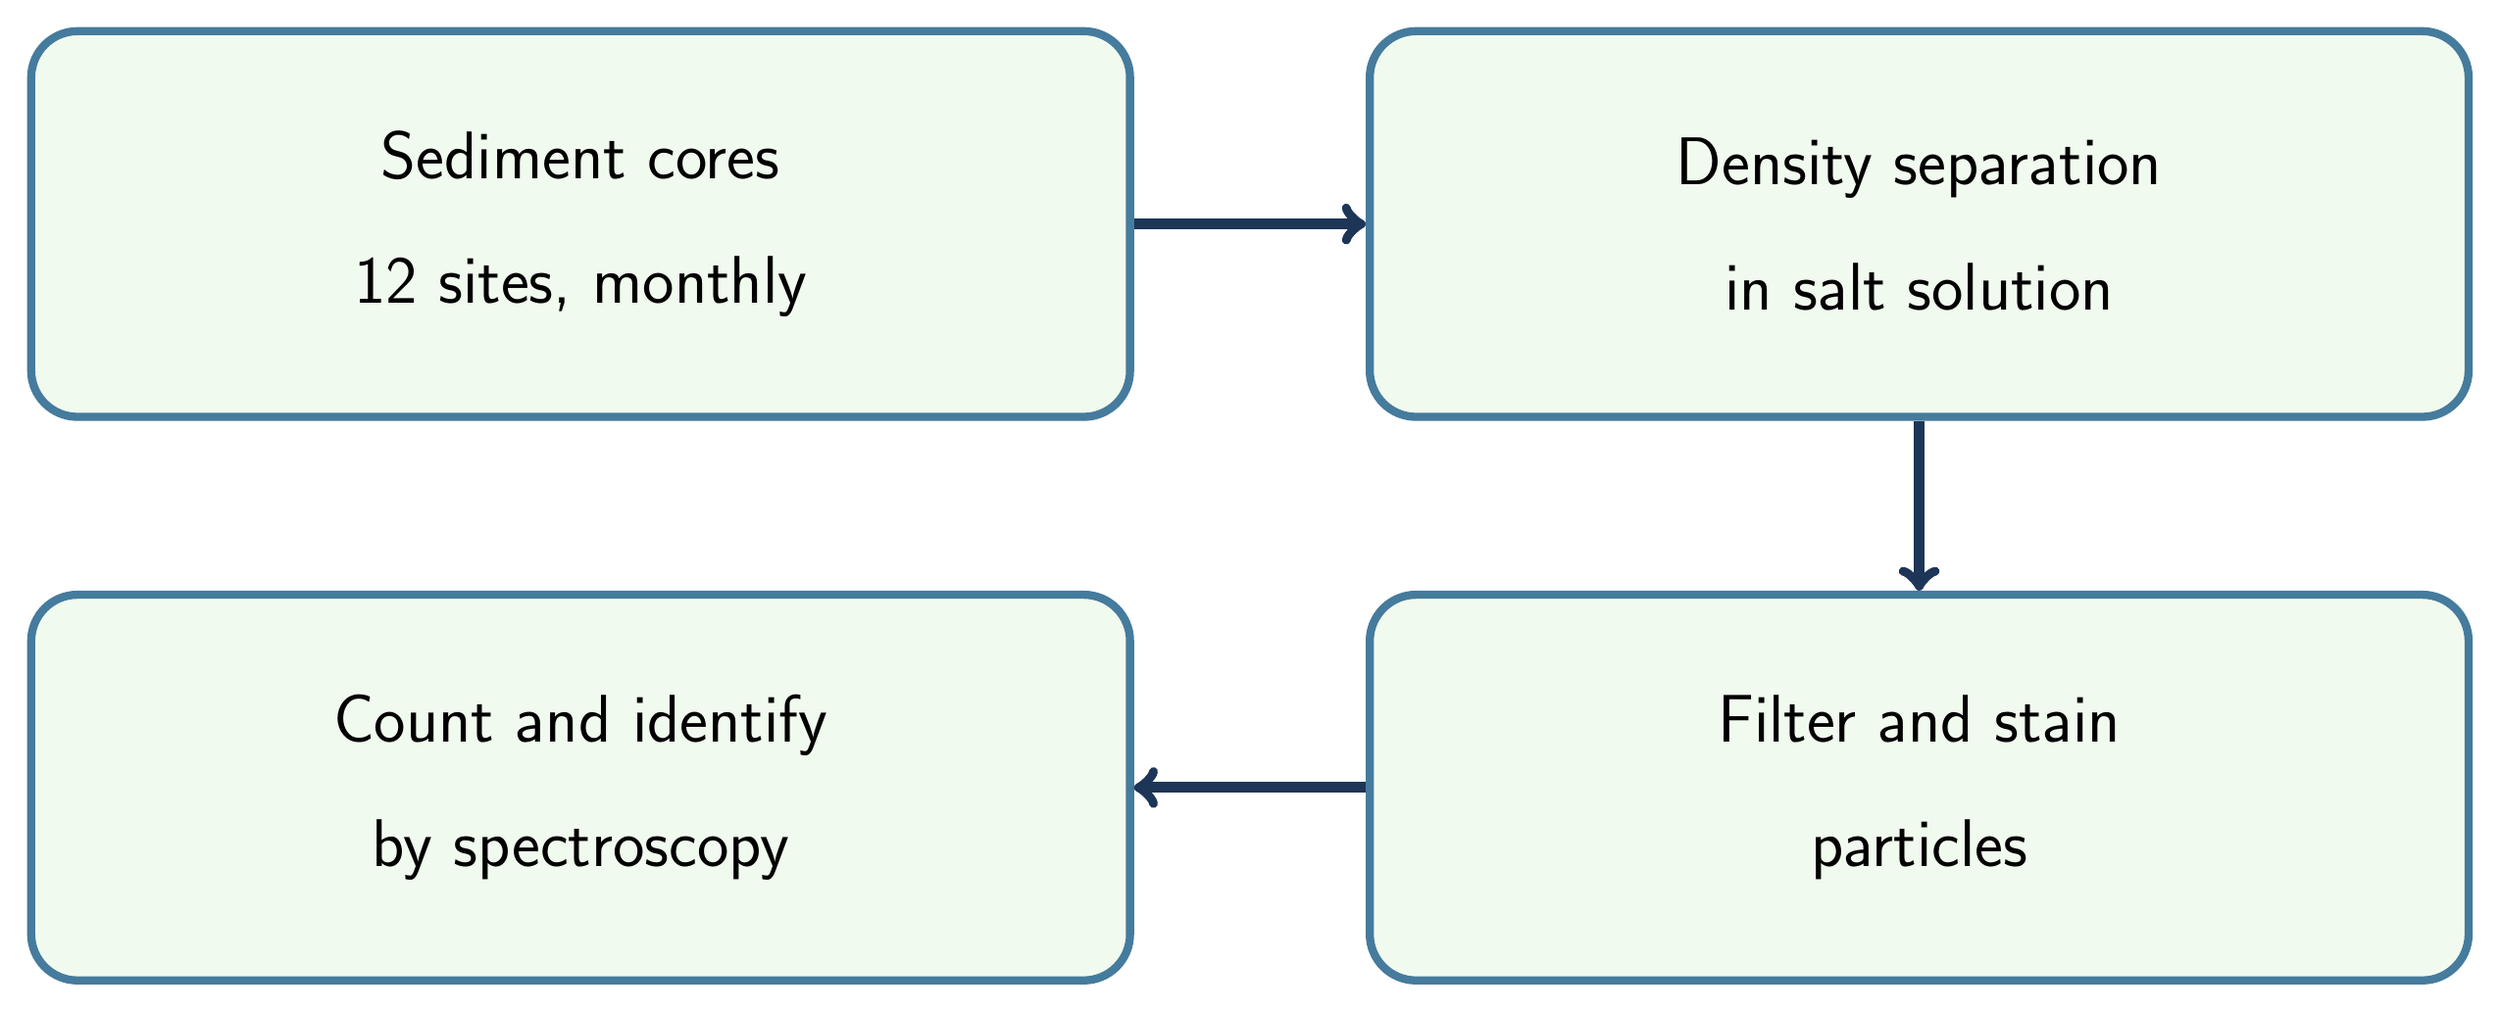
\begin{tikzpicture}[stage/.style={draw=secondary, line width=3pt, rounded corners=6mm, fill=light,
        text width=140mm, align=center, minimum height=50mm, font=\bodysize}, arr/.style={->, line width=4pt, primary}]
      \node[stage] (a) {Sediment cores\\12 sites, monthly};
      \node[stage, right=30mm of a] (b) {Density separation\\in salt solution};
      \node[stage, below=22mm of b] (c) {Filter and stain\\particles};
      \node[stage, left=30mm of c] (d) {Count and identify\\by spectroscopy};
      \draw[arr] (a) -- (b);
      \draw[arr] (b) -- (c);
      \draw[arr] (c) -- (d);
    \end{tikzpicture}
    \par\raggedright
    Counts are reported per kilogram of dry sediment. We model the monthly count $y_t$ as
    \[ \log y_t = \beta_0 + \beta_1\, Q_{t-1} + \varepsilon_t , \]
    where $Q_{t-1}$ is the peak discharge in the previous month.
  \end{panel}
\end{minipage}\hfill
\begin{minipage}[t]{0.485\linewidth}
  \vspace{0pt}
  \begin{panel}{Results}
    \textbf{Counts fall sharply after floods.} Mean particles per kg at lowland and upland sites:
    \par\centering
    % Edit the coordinates to plot your own monthly data.
    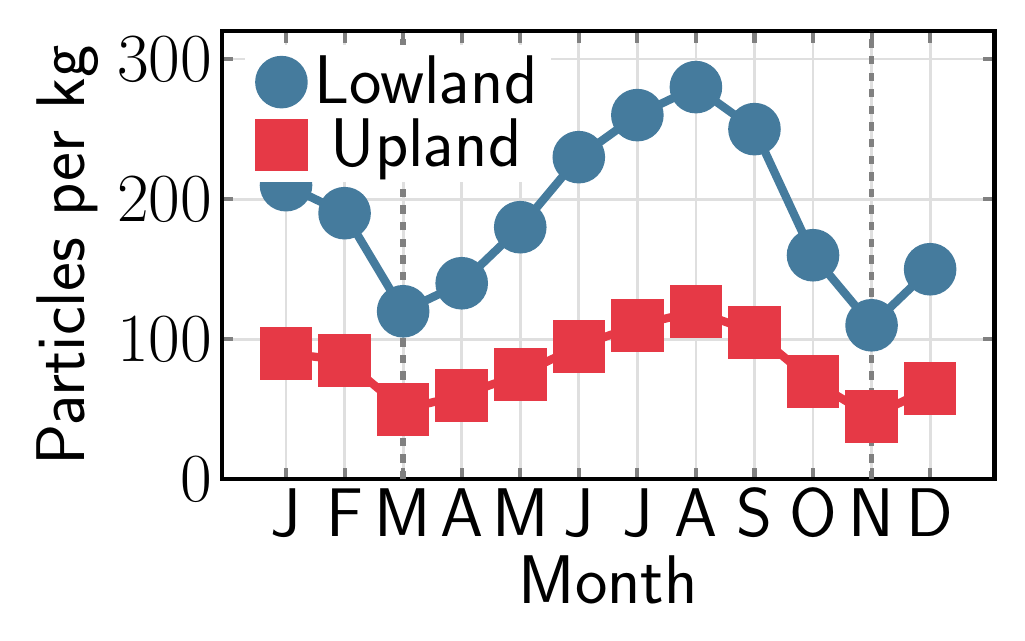
\begin{tikzpicture}
      \begin{axis}[posterplot, xlabel={Month}, ylabel={Particles per kg},
          xtick={1,...,12}, xticklabels={J,F,M,A,M,J,J,A,S,O,N,D},
          legend style={font=\smallsize, draw=none, fill=white}, legend pos=north west, ymin=0, ymax=320]
        \addplot[secondary, mark=*, mark size=8pt] coordinates {
          (1,210) (2,190) (3,120) (4,140) (5,180) (6,230) (7,260) (8,280) (9,250) (10,160) (11,110) (12,150)};
        \addlegendentry{Lowland}
        \addplot[accent, mark=square*, mark size=8pt] coordinates {
          (1,90) (2,85) (3,50) (4,60) (5,75) (6,95) (7,110) (8,120) (9,105) (10,70) (11,45) (12,65)};
        \addlegendentry{Upland}
        \draw[line width=2pt, dashed, gray] (axis cs:3,0) -- (axis cs:3,320);
        \draw[line width=2pt, dashed, gray] (axis cs:11,0) -- (axis cs:11,320);
      \end{axis}
    \end{tikzpicture}
    \par\smallsize Dashed lines mark the two flood peaks.
    \par\bodysize\raggedright
    \vspace{10mm}
    \textbf{Polymer types found} (share of all particles):
    \par\centering
    \begin{tabular}{lrr}
      \toprule
      Polymer & Lowland & Upland \\
      \midrule
      Polyethylene & 41\% & 36\% \\
      Polypropylene & 27\% & 30\% \\
      Polyester fibres & 22\% & 25\% \\
      Other & 10\% & 9\% \\
      \bottomrule
    \end{tabular}
  \end{panel}

  \begin{panel}{Conclusions}
    \begin{tcolorbox}[colback=accent!10, colframe=accent, boxrule=3pt, arc=5mm, left=10mm, right=10mm]
      \bfseries A single annual sample can misjudge sediment plastic by a factor of two.
    \end{tcolorbox}
    \begin{itemize}
      \item Counts drop by about 45\% after each flood peak.
      \item Sediment refills within three to four months.
      \item Monitoring should sample before and after flood season.
    \end{itemize}
  \end{panel}

  \begin{panel}{Next steps}
    \begin{itemize}
      \item Add weekly sampling during the flood months.
      \item Track where flushed particles settle downstream.
      \item Share the protocol with regional monitoring agencies.
    \end{itemize}
  \end{panel}

  \begin{panel}{References and contact}
    \smallsize
    \begin{enumerate}[label={[\arabic*]}]
      \item Author, A. and Writer, B. Plastic transport in rivers. \emph{Example Journal of Water}, 12:1, 2023.
      \item Researcher, C. Sediment sampling methods. \emph{Methods in Example Ecology}, 8:44, 2024.
      \item Scholar, D. et al. Polymer identification at scale. \emph{Example Analytical Letters}, 3:9, 2025.
    \end{enumerate}
    Contact: ana.beltran@example.org\\
    Funded by the Example Research Council, grant 00000.
  \end{panel}
\end{minipage}

\end{document}
